\section{Introduction}
\begin{frame}{\insertsection}
    \begin{itemize}
        \item Security of Unmanned Aerial Vehicles (UAVs)
        \item Increased popularity
        \item Military and non-military
    \end{itemize}
\end{frame}

\begin{frame}{\insertsection}
    \begin{itemize}
        \item Government, law enforcement, fire fighting, emergency rescue, and so on...
    \end{itemize}
    
    \begin{figure}[h]
        \centering
        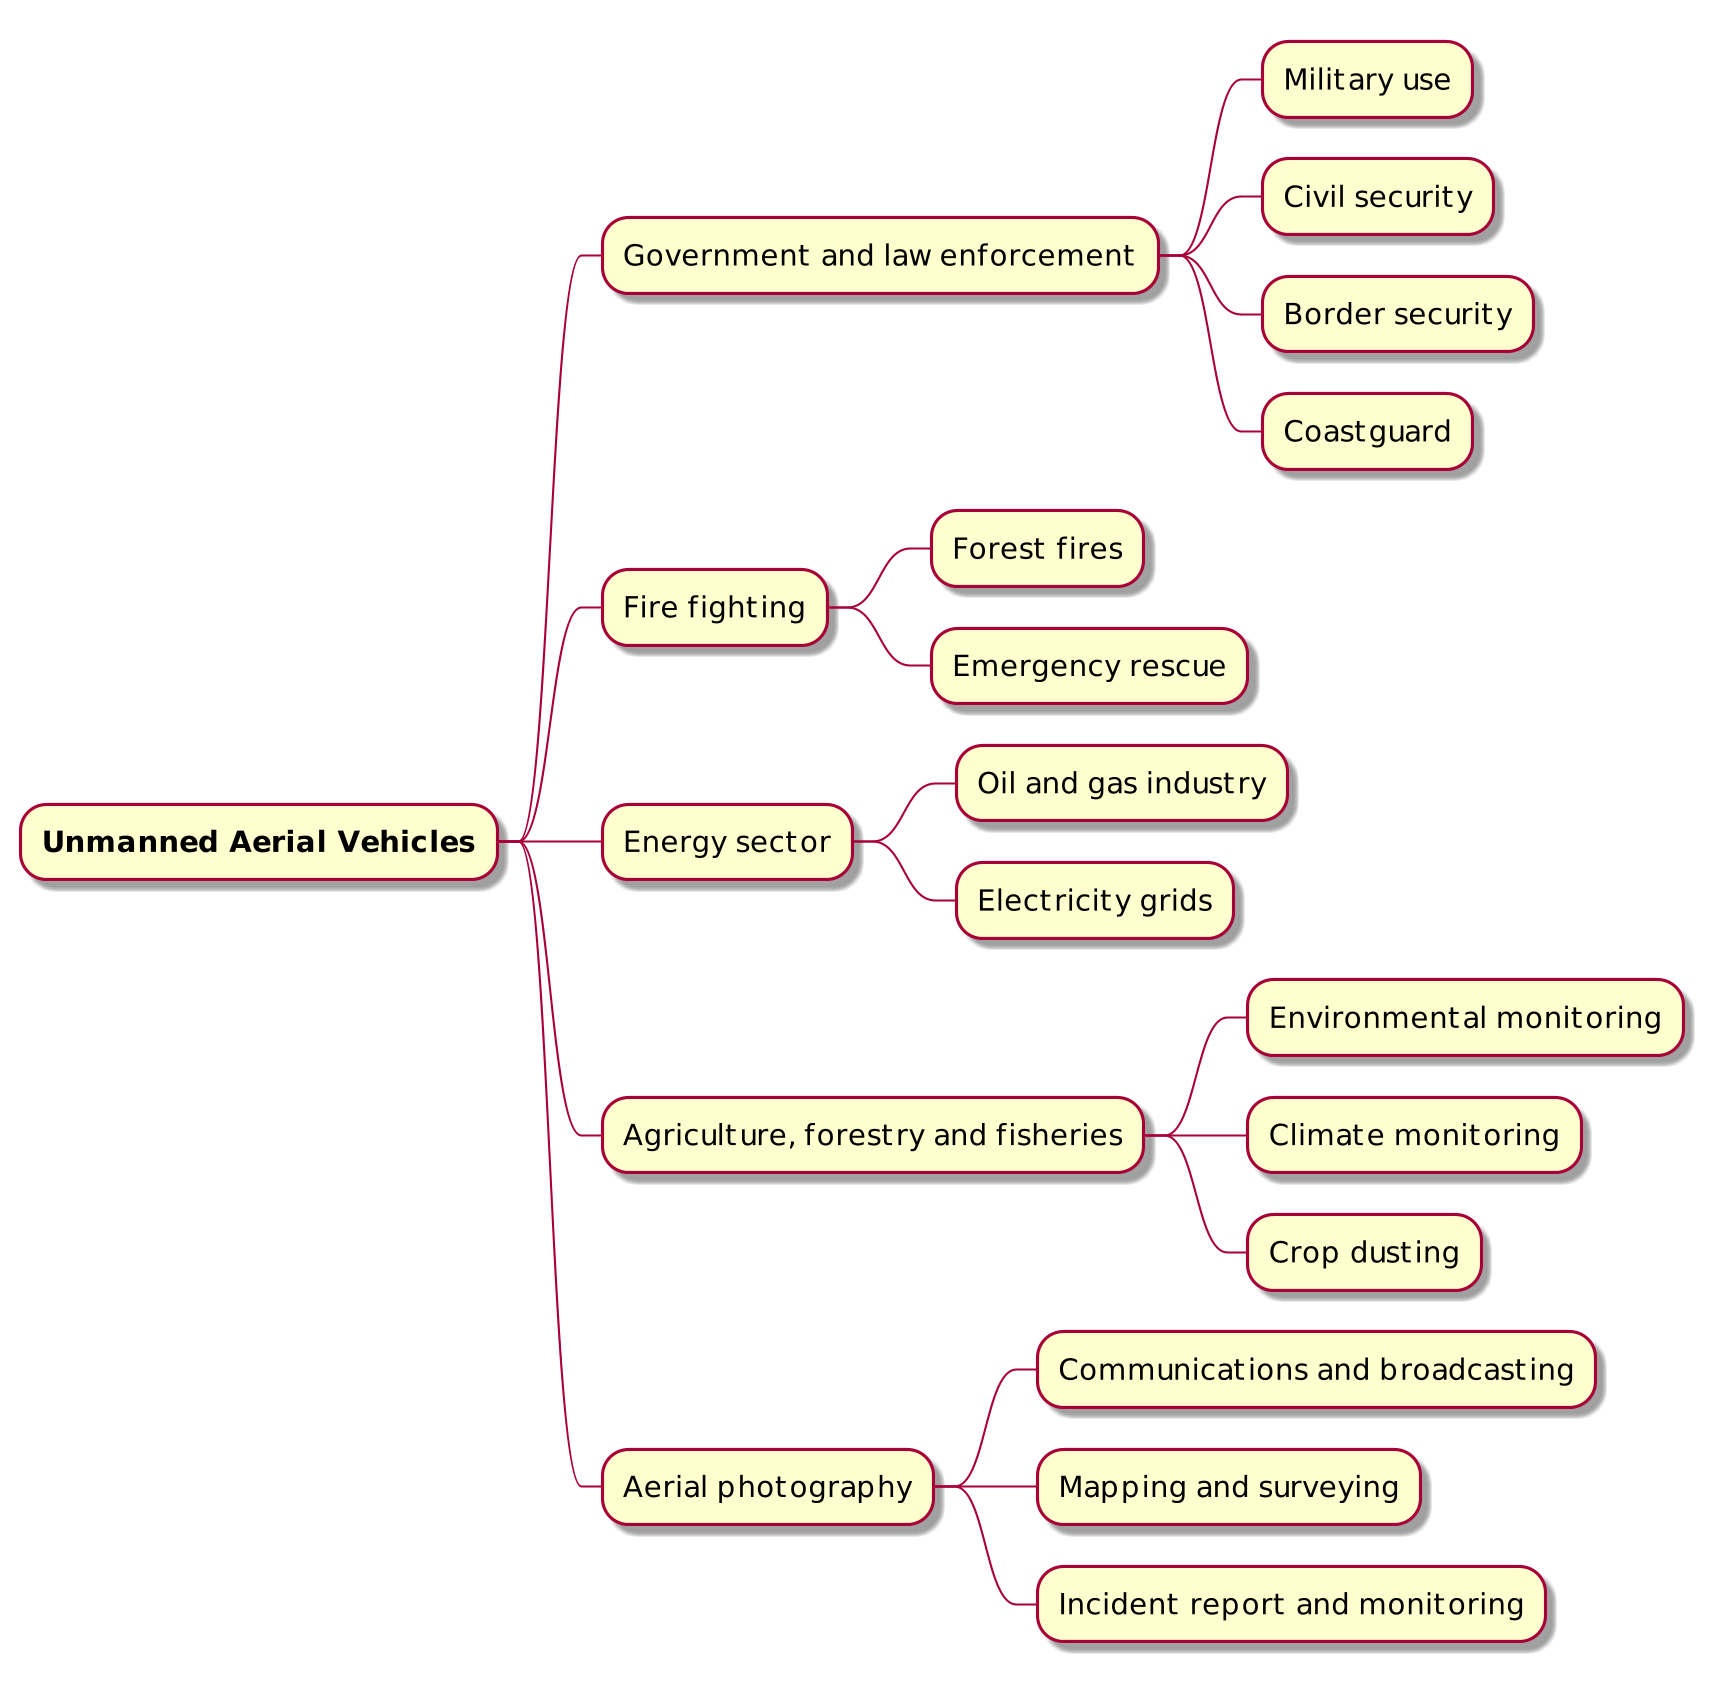
\includegraphics[width=7cm]{img/usage.png}
        \label{fig:usage}
    \end{figure}
\end{frame}

\subsection{Anatomy of a UAV}
\begin{frame}{\insertsubsection}
    \begin{itemize}
        \item Flight controller deployed at the center
        \item Electronic Speed Controllers (ESCs)
        \item Radio interface
        \item GNSS (GPS), radar antenna, multiband data-link antenna
    \end{itemize}
    
    \begin{figure}[h]
        \centering
        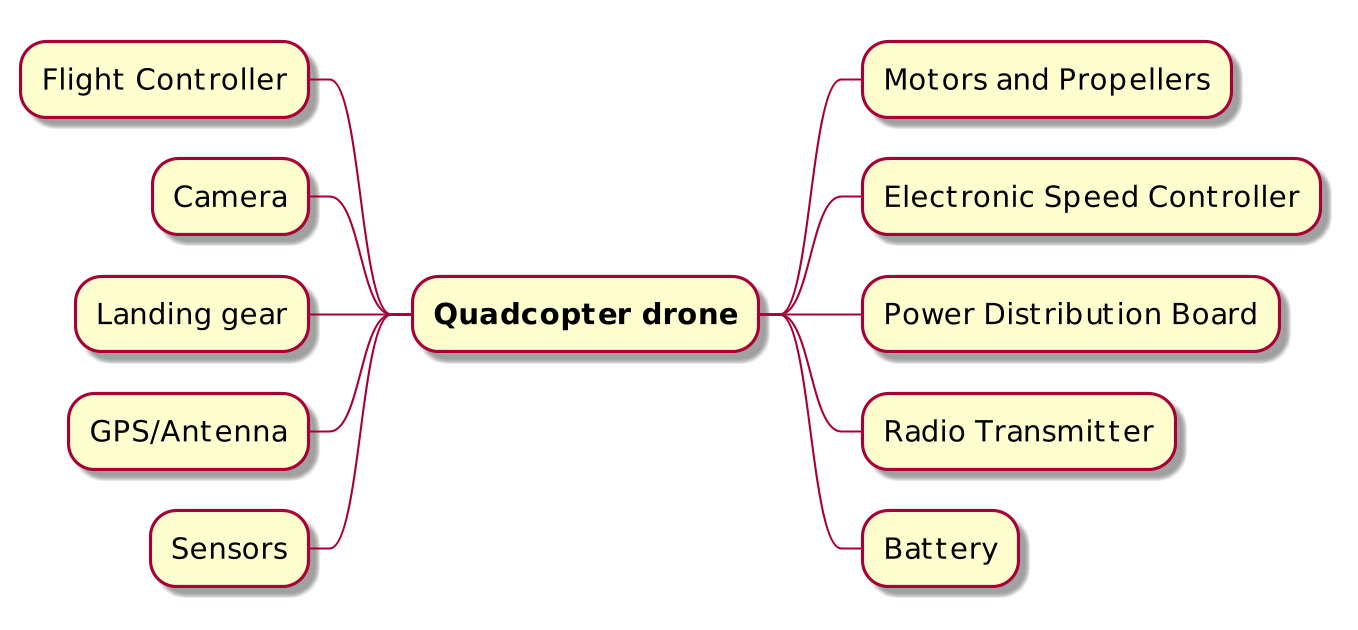
\includegraphics[width=10cm]{img/quadcopter.png}
        \label{fig:quadcopter}
    \end{figure}
\end{frame}

\section{History of UAV security exploits and cyber attacks}
\begin{frame}{\insertsection}
    \begin{itemize}
        \item \url{https://www.csmonitor.com/World/Middle-East/2011/1215/Exclusive-Iran-hijacked-US-drone-says-Iranian-engineer}
    \end{itemize}
    
    \begin{figure}[h]
        \centering
        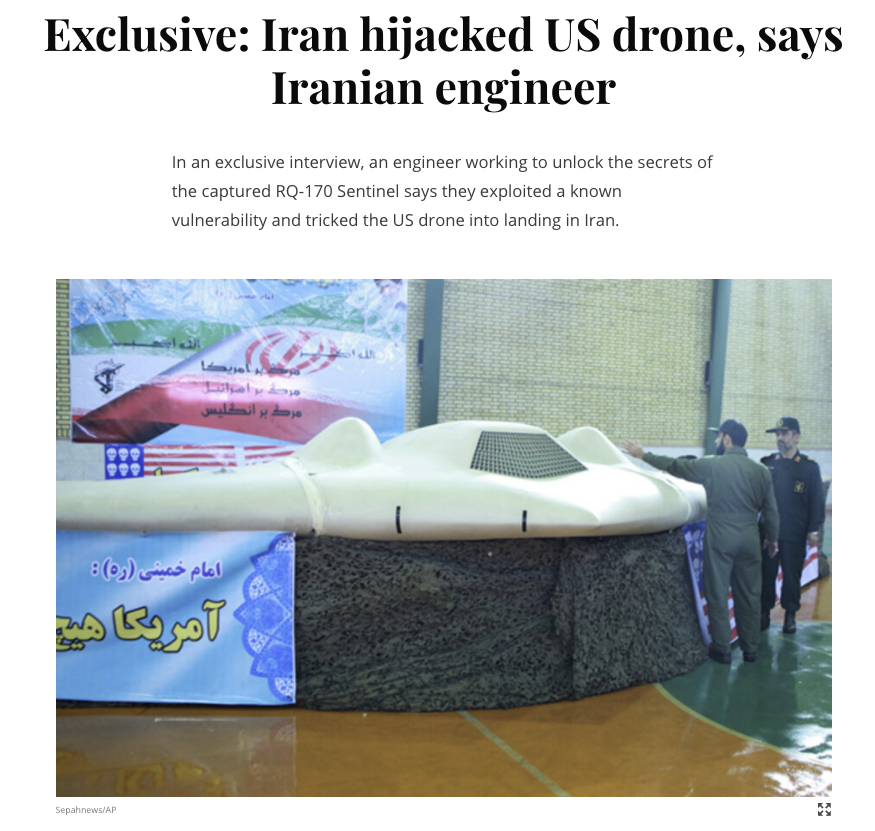
\includegraphics[width=7cm]{img/iran.png}
        \label{fig:iran}
    \end{figure}
\end{frame}

\begin{frame}{\insertsection}
    \begin{itemize}
        \item \url{https://www.theguardian.com/world/2009/dec/17/skygrabber-american-drones-hacked}
    \end{itemize}
    
    \begin{figure}[h]
        \centering
        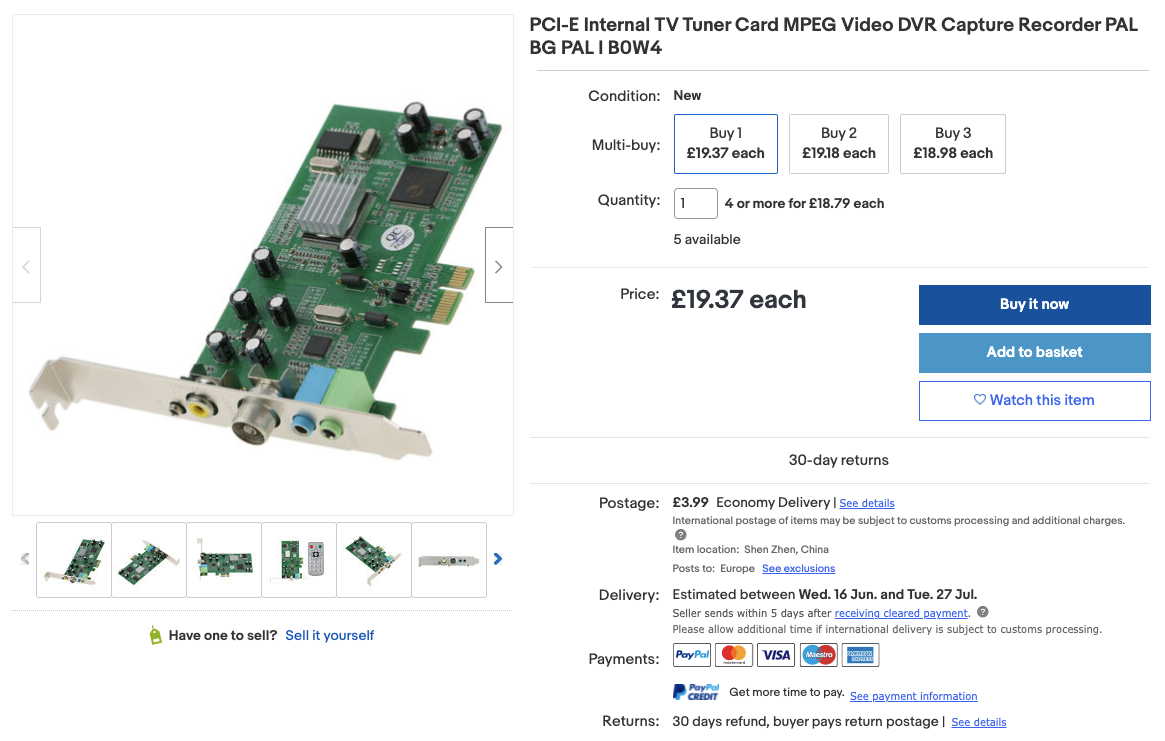
\includegraphics[width=10cm]{img/kort.png}
        \label{fig:iran}
    \end{figure}
\end{frame}

\section{Threats and vulnerabilities}
\begin{frame}{\insertsection}
    \begin{itemize}
        \item Hardware attacks
        \item Software attacks
        \item Fault injection and exploitation
        \item Communication attacks
    \end{itemize}
\end{frame}

\subsection{Cyber-physical attack surfaces}
\begin{frame}{\insertsubsection}
    \begin{itemize}
        \item Many attack surfaces exist in the cyber-physical domain
        \item Changes in the physical domain, and vice versa
        \item Massive consequences
        \item Manipulation of sensors and improper UAV navigation
        \vspace{0.5cm}
        \item Navigation (GPS), fault handling, network layer
        \item Data-driven systems
    \end{itemize}
\end{frame}

\section{Common attack methods}
\begin{frame}{\insertsection}
    \begin{itemize}
        \item Sniffing attack
        \item Spoofing and man-in-the-middle attack
        \item Jamming and DoS attack
    \end{itemize}
\end{frame}

\subsection{Sniffing attack}
\begin{frame}{\insertsubsection}
    \begin{itemize}
        \item Monitoring the communication channel
        \item Extract or "sniff" information through this channel
        \item Good key management and distribution
    \end{itemize}
\end{frame}

\subsection{Spoofing and man-in-the-middle attack}
\begin{frame}{\insertsubsection}
    \begin{itemize}
        \item Insert your own communication or messages
        \item Modify existing messages
        \item Compromise integrity of the UAV communication
    \end{itemize}
\end{frame}

\subsection{Jamming and DoS attack}
\begin{frame}{\insertsubsection}
    \begin{itemize}
        \item Denial of Service
        \item Flooding information with noise
        \item Compromises the availability of the UAV
        \item Hard to find solutions
        \item Add authentication to filter out malicious traffic
    \end{itemize}
\end{frame}

\section{Conclusion}
\begin{frame}{\insertsection}
    \begin{itemize}
        \item Increasing popularity
        \item Still many issues in regard to security and cyber crime
        \item A new trend among cyber criminals, many different attack vectors
        \item Many unknown security challenges ahead
        \item Phishing attempts, social engineering
    \end{itemize}
\end{frame}

\section{References}
\begin{frame}{\insertsection}
    \begin{itemize}
        \item \url{https://doi.org/10.1016/j.iot.2020.100218}
        \item \url{https://doi.org/10.1109/NTMS.2018.8328747}
        \item \url{https://doi.org/10.1109/ICPICS50287.2020.9201954}
        \item \url{https://publications.ffi.no/nb/item/asset/dspace:6791/20-01289.pdf}
        \vspace{0.5cm}
        \item More in the portfolio report...
    \end{itemize}
\end{frame}
